%!TEX root = documentation.tex

\chapter{Master}

\section{About the Master} % (fold)
\label{sec:about_the_master}

The master is written in Java and uses the jamod Library\footnote{\url{http://jamod.sourceforge.net/}} for the communication with the sensors using the modbus protocol. The view is created with the SWT Library\footnote{\url{http://www.eclipse.org/swt/}}. 
The description of the master is separated in several parts:
\begin{itemize}
	\item View (see \ref{sec:view})
	\item Configuration (see \ref{sec:configuration})
	\item Stations  (see \ref{sec:stations})
	\item History (see \ref{sec:history})
\end{itemize}

Before the collection process of the measurement values can be started it's necessary to create a configuration. In this configuration all sensors are defined. A sensor must be added to the master before it can be used. Each sensor has an individual name and ip address. In this context it's referred as a station. In the configuration phase it's necessary to specify the kind of data the stations collect. The data that is transferred from the station to the master is called Input Parameter. To configure the sensor it's possible to define Configuration Parameters. These values are transferred from the master to the sensor. To map the parameters to the memory in the station they must be bound to addresses. This happens individually for each station. So it's possible to collect different data from different stations. It's also possible to configure the kind of plots that are generated (see \ref{sub:plots}).

After the configuration of the stations the collection process can be started. Each station is polled in its own thread. One collector thread collects the data from the station threads, generates a text file with the information about the current values from the stations and draws the plots. The time between the polling of the stations and between generation of the output files can also be configured. As soon as the current day changes the values from the last day are aggregated to a history value. The values from the station are kept for two days so it's possible to build a plot based on hourly data from the last day. 

% section about_the_master (end)

\section{View} % (fold)
\label{sec:view}

The view is created with the help of SWT. SWT uses the OS drawing APIs to draw the widgets. So the look and feel of the application is very good integrated in the OS it runs on. 

\subsection{Screenshots} % (fold)
\label{sub:screenshots}
See Figure~\ref{fig:parameter}, \ref{view1}, \ref{fig:stations} (Page~\pageref{fig:stations}) and \ref{fig:data} (Page~\pageref{fig:data}) for screenshots of the master.

\begin{figure}[ht]
    \centering
    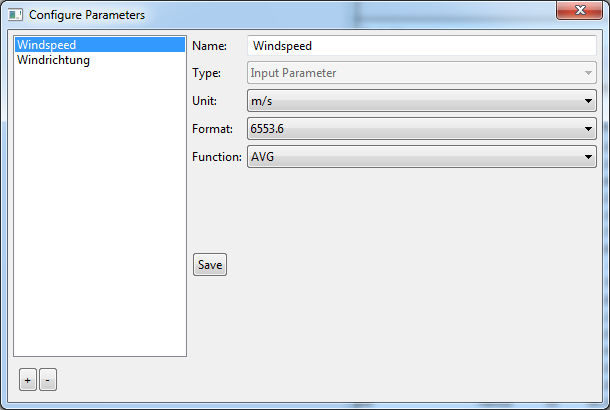
\includegraphics[width=0.8\linewidth]{master/parameters.jpg}
    \caption{Adding/editing of the parameters}
    \label{fig:parameter}
\end{figure} 

\begin{figure}
     \centering 
     \subfloat[Quick overview of the stations and their status]{\label{fig:main} 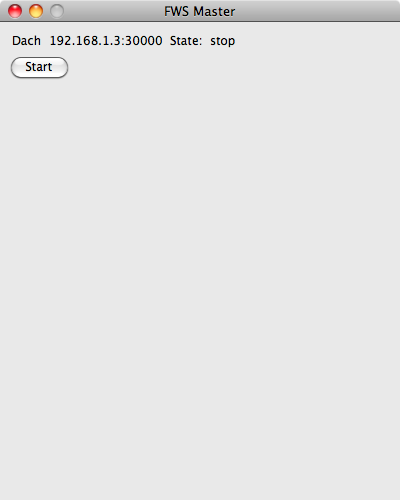
\includegraphics[width=0.4\linewidth]{master/mainview.png}} 
      \qquad
     \subfloat[Configuration of the basic settings]{\label{fig:settings} 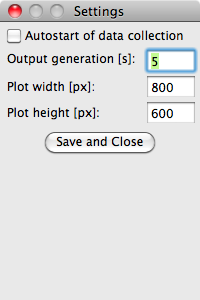
\includegraphics[width=0.4\linewidth]{master/settings.png}}
      \qquad
      \subfloat[Add new Station]{\label{fig:add} 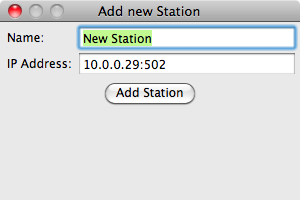
\includegraphics[width=0.4\linewidth]{master/add.png}}
     \caption{Screenshots of FWS Master} 
     \label{view1}
\end{figure}


\begin{figure}[p]
    \centering
    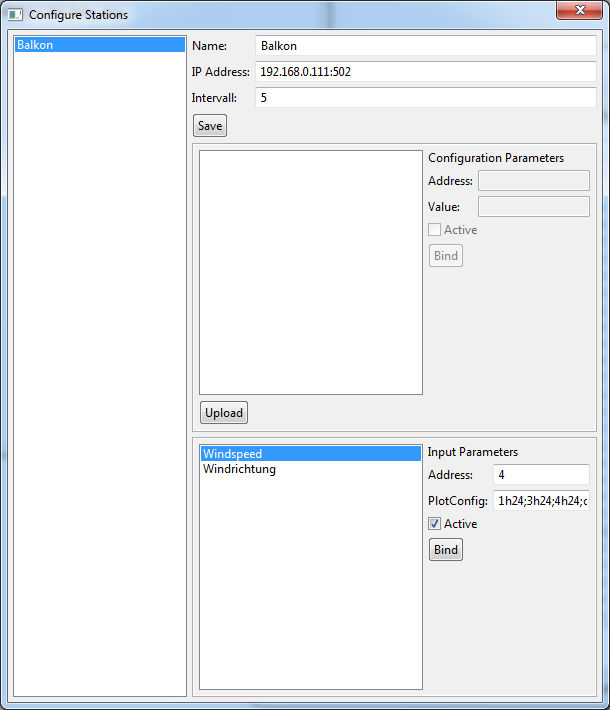
\includegraphics[width=0.8\linewidth]{master/stations.jpg}
    \caption{Editing station specific settings. The parameter bindings are also set here}
    \label{fig:stations}
\end{figure}

\begin{figure}[p]
    \centering
    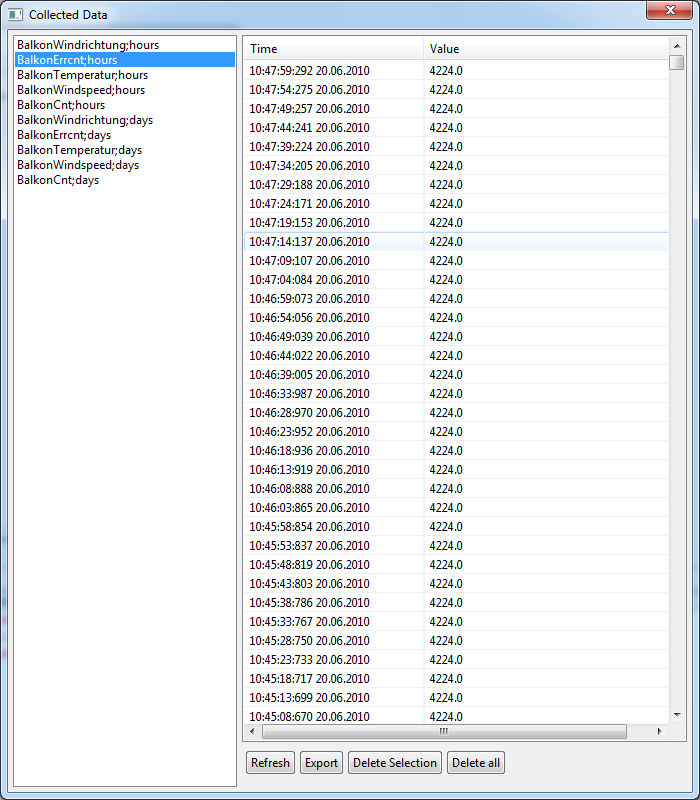
\includegraphics[width=0.8\linewidth]{master/viewdata.jpg}
    \caption{Shows the currently collected and saved data}
    \label{fig:data}
\end{figure}
% subsection screenshots (end)
\newpage
\section{Configuration} % (fold)
\label{sec:configuration} 
%TODO enabled wenn vorhanden
The views that support the configuration are \ref{fig:add}, \ref{fig:settings}, \ref{fig:parameter} and \ref{fig:stations}.

The result of the configuration phase is an XML file with all settings in it. The location of this file is OS dependent. 
\begin{itemize}
    \item \textbf{OS X}: /Users/\{username\}/Library/Application Support/FWSMaster/settings.xml
    \item \textbf{Linux}: \textasciitilde /.fws\_master/settings.xml
    \item \textbf{Windows}: C:\textbackslash \{User Dir\} \textbackslash .fws\_master \textbackslash settings.xml
\end{itemize}

See example in Listing \ref{code:settings}

{\C \lstinputlisting[language=xml,breaklines=true,caption={Sample settings file},label=code:settings,frame=tlRB]{master/settings.xml} }

\subsection{Parameters} % (fold)
\label{sub:parameters}
There are two types of parameters. Input Parameters and Configuration Parameters. Each parameter has a unique name and a boolean value if it's enabled. The name is the identifier of the parameter so it has to be unique. Beside of these common attributes the Configuration and Input Parameters have further attributes. The parameters must be assigned to station addresses. This process is referred as binding a parameter to a station. To bind a parameter to a station, the user must define the address on the station where the parameter is saved.

\subsubsection{Input Parameter} % (fold)
\label{ssub:input_parameter}
Additional attributes of an Input Parameter:
\begin{itemize}
	\item Unit
	\item Format
	\item History Function
\end{itemize}

\paragraph{Unit} % (fold)
\label{par:unit}
The Unit is just used for the description in the generated files. Available units are:
\begin{itemize}
	\item speed $\frac{m}{s}$
	\item speed $\frac{km}{h}$
	\item frequenzy $Hz$
	\item direction
	\item temperature $^\circ C$
\end{itemize}

% paragraph unit (end)

\paragraph{Format} % (fold)
\label{par:format}
The transferred value from the station is a 16 bit integer value. To be able to display floating point numbers it's possible to set the output format to the desired form. Example: The temperature equals $23.3 ^\circ C$. The station measures the temperature and converts it to $233$. This integer value is transmitted to the master. The master converts the number back to the desired format. So this example would result in $23.3$.

\paragraph{History Function} % (fold)
\label{par:histfunc}
There are three different history functions available. For more details about these functions and how they are used please read \ref{sec:history}.
\label{par:history_function}
\begin{itemize}
    \item average
    \item minimum
    \item maximum
\end{itemize}
% paragraph history_function (end)
% paragraph format (end)
% subsubsection input_parameter (end)

\subsubsection{Configuration Parameter} % (fold)
\label{ssub:configuration_parameter}
Additional attributes of a Configuration Parameter:
\begin{itemize}
    \item value
\end{itemize}

\paragraph{Value} % (fold)
\label{par:value}
A configuration parameter is a value that is transferred from the master to the slave. The value that is transferred is saved in the attribute value. This value must be an 16 bit integer value.
% paragraph value (end)
% subsubsection configuration_parameter (end)

% subsection parameters (end)

\subsection{Plots} % (fold)
\label{sub:plots}
The plots are generated with the help of the jFreeChart Library \footnote{\url{http://www.jfree.org/jfreechart/}}.
The plots can be configured for every binding of input parameters. Each binding can have several plots assigned. It's also possible to plot more than one data into one plot. The plots are configured with a string. The simplest configuration looks like {\C h24;} With that configuration one plot is generated and the data for this plot are the values from the last 24 hours. The plots are generated in the output directory that can be set by the user.

It's possible to use different data ranges for the plots. To allow the user to choose one range there are three different time bases available:
\begin{itemize}
	\item c - current
	\item h - hours
	\item d - days
\end{itemize}

\paragraph{Current} % (fold)
\label{par:current}
Use the newest values for the plot. Currently this is only implemented for the wind direction. See example in figure \ref{fig:current}.
\begin{figure}[ht]
    \centering
    
\includegraphics[width=0.9\linewidth]{master/plot_examplec.png}
    \caption{Current wind direction plot}
    \label{fig:current}
\end{figure}
% paragraph current (end)

\paragraph{Hours} % (fold)
\label{par:hours}
Use the values of the last hours for the plot. The amount of the hours is specified in the plot configuration. It's the number after the timebase. Example of an 24 hour plot see figure \ref{fig:hours}.
\begin{figure}[ht]
    \centering
    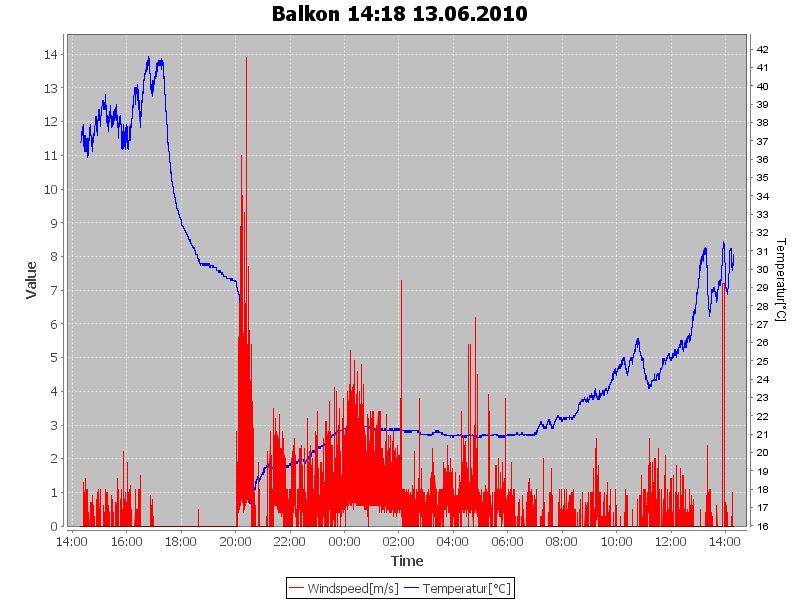
\includegraphics[width=0.9\linewidth]{master/plot_exampleh.png}
    \caption{Last 24 hours of two separate parameters in one plot}
    \label{fig:hours}
\end{figure}
% paragraph hours (end)

\paragraph{Days} % (fold)
\label{par:days}
Same plot as with the hours timebase but the values from the last days are used. For more details about the history see section \ref{sec:history}.
% paragraph days (end)

\subsubsection{Configuration Syntax} % (fold)
\label{ssub:configuration_syntax}
Each plot is specified by three different parts: [Number]CharacterNumber;

\paragraph{First Number: ID} % (fold)
\label{par:first_number_id}
This number is optional and controls if more than one input parameter is drawn in one plot. All configured plots with the same number are drawn in the same plot.
% paragraph first_number_id (end)
\paragraph{Character: Timebase} % (fold)
\label{par:character}
Defines the timebase. Explained in paragraphs above.
% paragraph character (end) 
\paragraph{Second Number: Amount of data} % (fold)
\label{par:number}
The second number defines how much data will be in the plot. {\C d4;} will plot the last four days.
% paragraph number (end)
\paragraph{End of Configuration} % (fold)
\label{par:end_of_configuration}
Each configuration must end with an {\C `;'}.
% paragraph end_of_configuration (end)

\paragraph{Example} % (fold)
\label{par:example}
For the configuration string {\C h24;1h24;d30;c1;d365;} following plots are generated:
\begin{itemize}
	\item Last 24 hours
	\item Last 24 hours with other data with ID 1 
	\item Last 30 days
	\item Current value
	\item Last 365 days
\end{itemize}

% paragraph example (end)
% subsubsection configuration_syntax (end)

\subsubsection{Detailed Information about the plots} % (fold)
\label{ssub:detailed_information_about_the_plots}
If two different datasets are plotted in one diagram two axis with separate scales will be generated. When more than two data sets should be drawn in one diagram they share one axis. So it's advisable to generate more plots with two datasets each to keep the diagrams tidy.

The direction parameters values are not connected with a line. Otherwise the diagrams would be complicated if the wind direction changes a lot.

The direction parameter values are mapped to a description of the direction. So $0^\circ$ results in N(orth) see figure \ref{fig:dir}
\begin{figure}[ht]
    \centering
    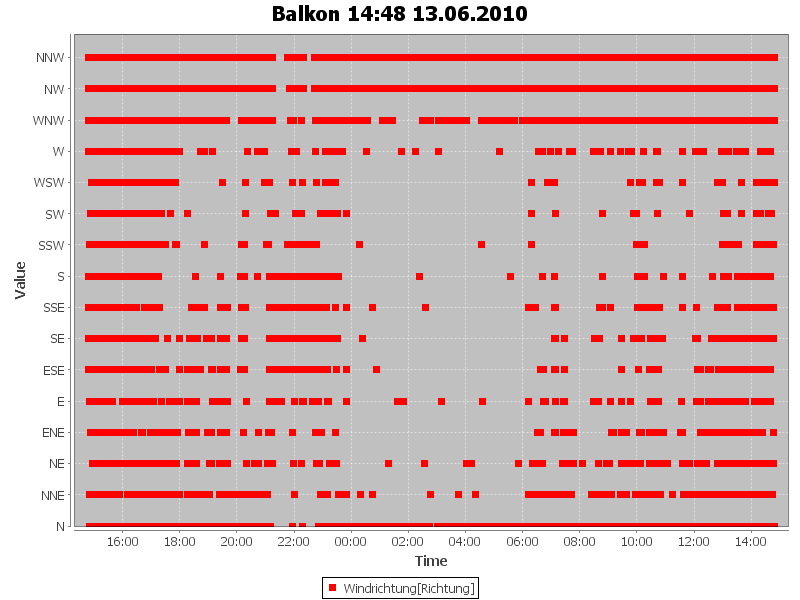
\includegraphics[width=0.9\linewidth]{master/plot_dir.png}
    \caption{Axis description of direction parameter}
    \label{fig:dir}
\end{figure}
% subsubsection detailed_information_about_the_plots (end)
% subsection plots (end)
% section configuration (end)

\section{Stations} % (fold)
\label{sec:stations}

After the stations are configured they are added to the station controller. This controller takes care for starting and pausing the station threads. 

\subsubsection{Transferring the Data} % (fold)
\label{ssub:getting_the_data}
Each station runs in it's own thread. This thread polls in its own interval the data values from the station. For each transmission a new TCP connection is opened. After the value has been transferred the connection gets closed. Each station has a list of measurements. A measurement consists of a timestamp and a value. These lists are collected from the Output Generation Thread. If a station is paused its thread gets suspended and waits for the wake up signal from the controller. 

The Modbus function that is used to transfer the data is read register.
% subsubsection getting_the_data (end)

\subsubsection{Transferring the configuration} % (fold)
\label{ssub:transferring_the_configuration}
When the user wants to upload a new configuration the station will call Write Register for each Configuration Parameter and reads back the answer of the station. If the answer equals the write register value the value is marked as transferred. A transferred value isn't uploaded again if it is unchanged.
% subsubsection transferring_the_configuration (end)
\subsubsection{Change the IP Address} % (fold)
\label{ssub:change_the_ip_address}
The IP Address represents a special configuration parameter. It is always mapped to the address 0 and 1 on the station. These two 16 bit registers are used to save the ip address. When the ip address has changed it's transferred to the station. After the successful transmission of the two values the new ip is saved. Otherwise the old ip is kept.
% subsubsection change_the_ip_address (end)


\subsubsection{Collecting the Data} % (fold)
\label{ssub:collecting_the_data}
A data collector thread runs in background an collects the data from all the stations. For each station/parameter combination a distinct list is kept with all the recent values in it. Before saving the measurements they are converted into a simpler data type that can be serialized and does not have references to other classes.

In the collector thread the text file is generated that contains the information about the current status of the stations. Each station is represented in this file. The information written in this file are the current values of the Input Parameters bound to that station. This value is the average of the measurements since the last run of the collector. To be able to see whether the value changes the standard deviation is calculated and written to the output. For example result file see listing \ref{code:result}. 
For each parameter a new line is started in the result file. Syntax is {\C name[unit]:value;standard deviation;}

{\C \lstinputlisting[breaklines=true,caption={Sample result file},label=code:result,frame=tlRB]{master/result.txt} }

% subsubsection collecting_the_data (end)
% section stations (end)

\section{History} % (fold)
\label{sec:history}
The collector adds the measurements to the history controller. This controller converts the values to the entries in the history. Each input parameter has two histories. One short term history and one long term history. 
\subsection{Short term history} % (fold)
\label{sub:short_term_history}
In the short term history there are the history entries from the last two days. This history is queried when plotting a diagram with the `h' timebase. To this list all new measurements are added as soon as new data arrive from the collector. During this phase it's checked whether the day has changed since the last time new measurements have been added. If that is the case the day is transferred to the long term history. There are at least the last 24 hours in the short term history.
% subsection short_term_history (end)

\subsection{Long term history} % (fold)
\label{ssub:long_term_history}
As soon as a new day has started the past day gets transferred to the long term history. To avoid to many values in this list one representing value is calculated for the day. This happens with one of the history functions listed in \ref{par:histfunc}. During the calculation of the history value all measurements older than the last day are removed from the short day history. The representing value is added to the long term history.
% subsection long_term_history (end)

\subsection{Storage of the history} % (fold)
\label{sub:storage_of_the_history}
The short and long term history are serialized to the hard disk. After new data have been added to the history it's saved to the hard disk. To prevent the user closing the master during the I/O operations a semaphore is used. \footnote{Without that semaphore we often had corrupted history files because the master closed at a critical instant.}

An old history is kept to prevent loosing the history if the master crashes during writing the history. Before saving the history the thread locks the semaphore. After that it renames the current history to another filename. After that the new history is saved. The history is saved now so the semaphore is released.

If an exception arises during loading the history the master tries to load the old history file. If that also results in an exception a new history is created.
% subsection storage_of_the_history (end)
% section history (end)

\section{Implementation details} % (fold)
\label{sec:implementation_details}
The source code can be downloaded at github\footnote{\url{http://www.github.com/schugabe/fws}}. The doc folder there contains the javadoc generated source code documentation.

In the following list you see which classes implement which functions. For a class diagram see figure \ref{fig:class_master}.

\begin{itemize}
    \item View: All classes that start with view
    \item Configuration: Parameter, InputParameter, ConfigParameter, StationInputBinding, StationConfigBinding, Station
    \item Save the configuration: PersistencePreferences, all classes with ContentHandler in their name
    \item Data collection: Station, MeasurementCollector, Measurement, StationInputBinding, MeasurementHistoryController, MeasurementHistory, MeasurementHistoryEntry
    \item Plotting and Output generation: MeasurementCollector, PlotBase, TimePlot, CurrentPlot
    \item ModBus: ModbusWrapper, Station
\end{itemize}

%TODO grafik aktualiserien
\begin{figure}[ht]
    \centering
    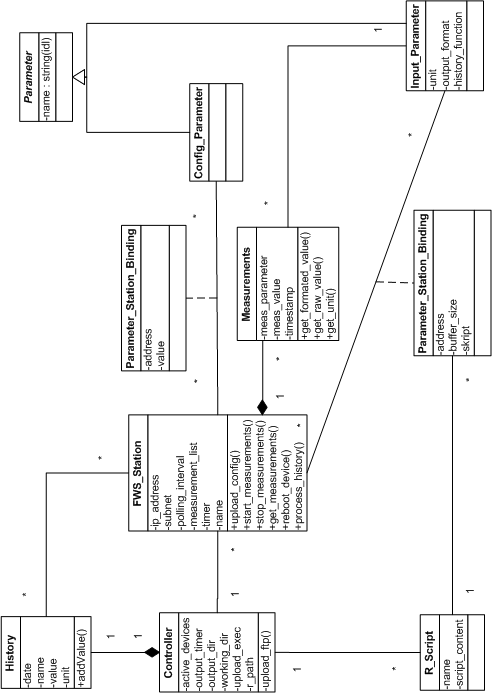
\includegraphics[width=\linewidth]{master/class.png}
    \caption{Class diagram of the master}
    \label{fig:class_master}
\end{figure}



% section implementation_details (end)